\documentclass[conference]{IEEEtran}

% --- パッケージ ---
\usepackage{amsmath,amssymb}
\usepackage{siunitx}
\usepackage{graphicx}
\usepackage[caption=false,font=footnotesize]{subfig}
\usepackage{tikz}
\usetikzlibrary{positioning,arrows.meta}
\usepackage{booktabs}
\usepackage{cite}
\usepackage{newtxtext,newtxmath} % Times系フォント

% 図まわりの間隔を調整(崩れ防止)
\setlength{\textfloatsep}{10pt plus 2pt minus 2pt}
\setlength{\floatsep}{8pt plus 2pt minus 2pt}
\setlength{\intextsep}{6pt plus 2pt minus 2pt}
\setlength{\abovecaptionskip}{3pt}

% 孤立行の防止
\clubpenalty=10000
\widowpenalty=10000

% 見出し直前の余白を少し空けるコマンド
\newcommand{\tightsecspace}{\vspace{0.3\baselineskip}}

\begin{document}

\title{Low-Cost Integration of 1.8-V FeFET on 0.18-$\mu$m CMOS:\\
+1 Mask and a Single ALD Tool, with Reliability Assessment}

\author{\IEEEauthorblockN{Shinichi Samizo}
\IEEEauthorblockA{Independent Semiconductor Researcher\\
Former Engineer at Seiko Epson Corporation\\
Email: shin3t72@gmail.com\\
GitHub: https://github.com/Samizo-AITL}
}

\maketitle

\begin{abstract}
Ferroelectric FETs (FeFETs) are promising CMOS-compatible embedded NVMs. 
This paper demonstrates a 1.8 V FeFET module integrated on a legacy 0.18~$\mu$m CMOS process with only one additional mask and a single ALD tool. 
Fabricated devices show endurance exceeding $10^5$ program/erase cycles and retention longer than 10 years at 85$^\circ$C. 
Reliability was characterized on FeCAP/FeFET structures: time-zero dielectric breakdown (TZDB), time-dependent dielectric breakdown (TDDB), endurance, and retention. 
The approach provides a cost-effective path to extend mature-node lifetimes and to enable embedded NVM for automotive/industrial/IoT, while high-temperature retention remains the key limiter.
\end{abstract}

\section{Introduction}
FeFETs based on HfO$_2$ have gained traction as CMOS-compatible NVMs. 
Most prior work targets advanced nodes; however, mature nodes ($\sim$0.18~$\mu$m) remain widely used in automotive/industrial markets where long supply lifetimes and low cost are critical. 
\textbf{This work contributes}: (i) a +1 mask low-cost module, (ii) only one ALD tool added to the line, (iii) a yield-friendly \textit{SRAM+FeFET} system usage model, and (iv) comprehensive reliability evidence on FeCAP/FeFET.

\section{Process Integration}
Baseline is a 0.18~$\mu$m CMOS platform (1.8 V core, optional 3.3 V I/O). 
The FeFET module is inserted after poly definition and salicide/RTA, requiring minimal line modification.

\subsection{Process Flow}
\begin{figure}[!t]
  \centering
  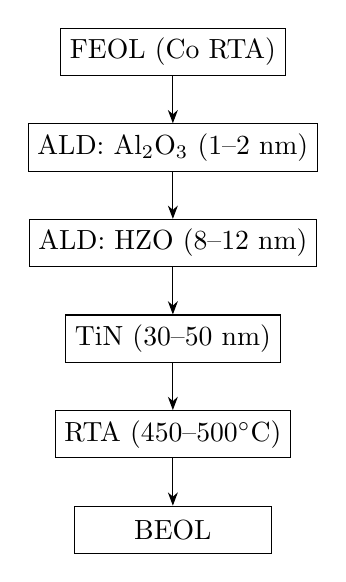
\begin{tikzpicture}[node distance=6mm, every node/.style={draw,rectangle,minimum width=25mm,minimum height=6mm},>=Stealth]
    \node (a) {FEOL (Co RTA)};
    \node (b) [below=of a] {ALD: Al$_2$O$_3$ (1--2 nm)};
    \node (c) [below=of b] {ALD: HZO (8--12 nm)};
    \node (d) [below=of c] {TiN (30--50 nm)};
    \node (e) [below=of d] {RTA (450--500$^\circ$C)};
    \node (f) [below=of e] {BEOL};
    \draw[->] (a) -- (b);
    \draw[->] (b) -- (c);
    \draw[->] (c) -- (d);
    \draw[->] (d) -- (e);
    \draw[->] (e) -- (f);
  \end{tikzpicture}
  \caption{Process flow of FeFET integration.}
  \label{fig:flow}
\end{figure}

\subsection{Cross Section}
\begin{figure}[!t]
  \centering
  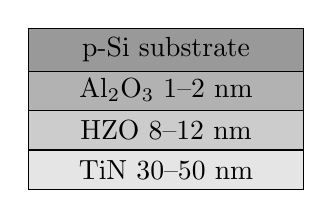
\begin{tikzpicture}
    \node[draw,fill=gray!20,minimum width=35mm,minimum height=5mm,anchor=south west] (tin) at (0,0) {TiN 30--50 nm};
    \node[draw,fill=gray!40,minimum width=35mm,minimum height=5mm,anchor=south west] (hzo) at (0,0.5) {HZO 8--12 nm};
    \node[draw,fill=gray!60,minimum width=35mm,minimum height=5mm,anchor=south west] (al) at (0,1.0) {Al$_2$O$_3$ 1--2 nm};
    \node[draw,fill=gray!80,minimum width=35mm,minimum height=5mm,anchor=south west] (si) at (0,1.5) {p-Si substrate};
  \end{tikzpicture}
  \caption{Cross section of HZO/Al$_2$O$_3$/TiN stack.}
  \label{fig:stack}
\end{figure}

\section{Devices and Methods}
Test structures include FeCAPs (flat/comb) and 100~$\mu$m $\times$ 100~$\mu$m FeFET cells. 
Programming used $\pm$2.3–2.7 V, 1–50 $\mu$s pulses. Keysight B1500A and a manual probe were used.

\textbf{Protocols}: TZDB: DC ramp $\approx$ 0.1 V/s at RT–125$^\circ$C. 
TDDB: constant-voltage stress at $\pm$2.3/2.5/2.7 V, 85$^\circ$C and 125$^\circ$C; Weibull fitting. 
Endurance: $\pm$2.5 V, 10 $\mu$s, 10 kHz up to $10^5$ cycles. 
Retention: 25$^\circ$C, 85$^\circ$C, 125$^\circ$C, with Arrhenius extrapolation.

\section{Results}
\subsection{TZDB}
Breakdown statistics indicate early-failure tails due to defects.

\begin{figure*}[!t]
  \centering
  \subfloat[TZDB distributions of FeCAPs.\label{fig:tzdb}]{
    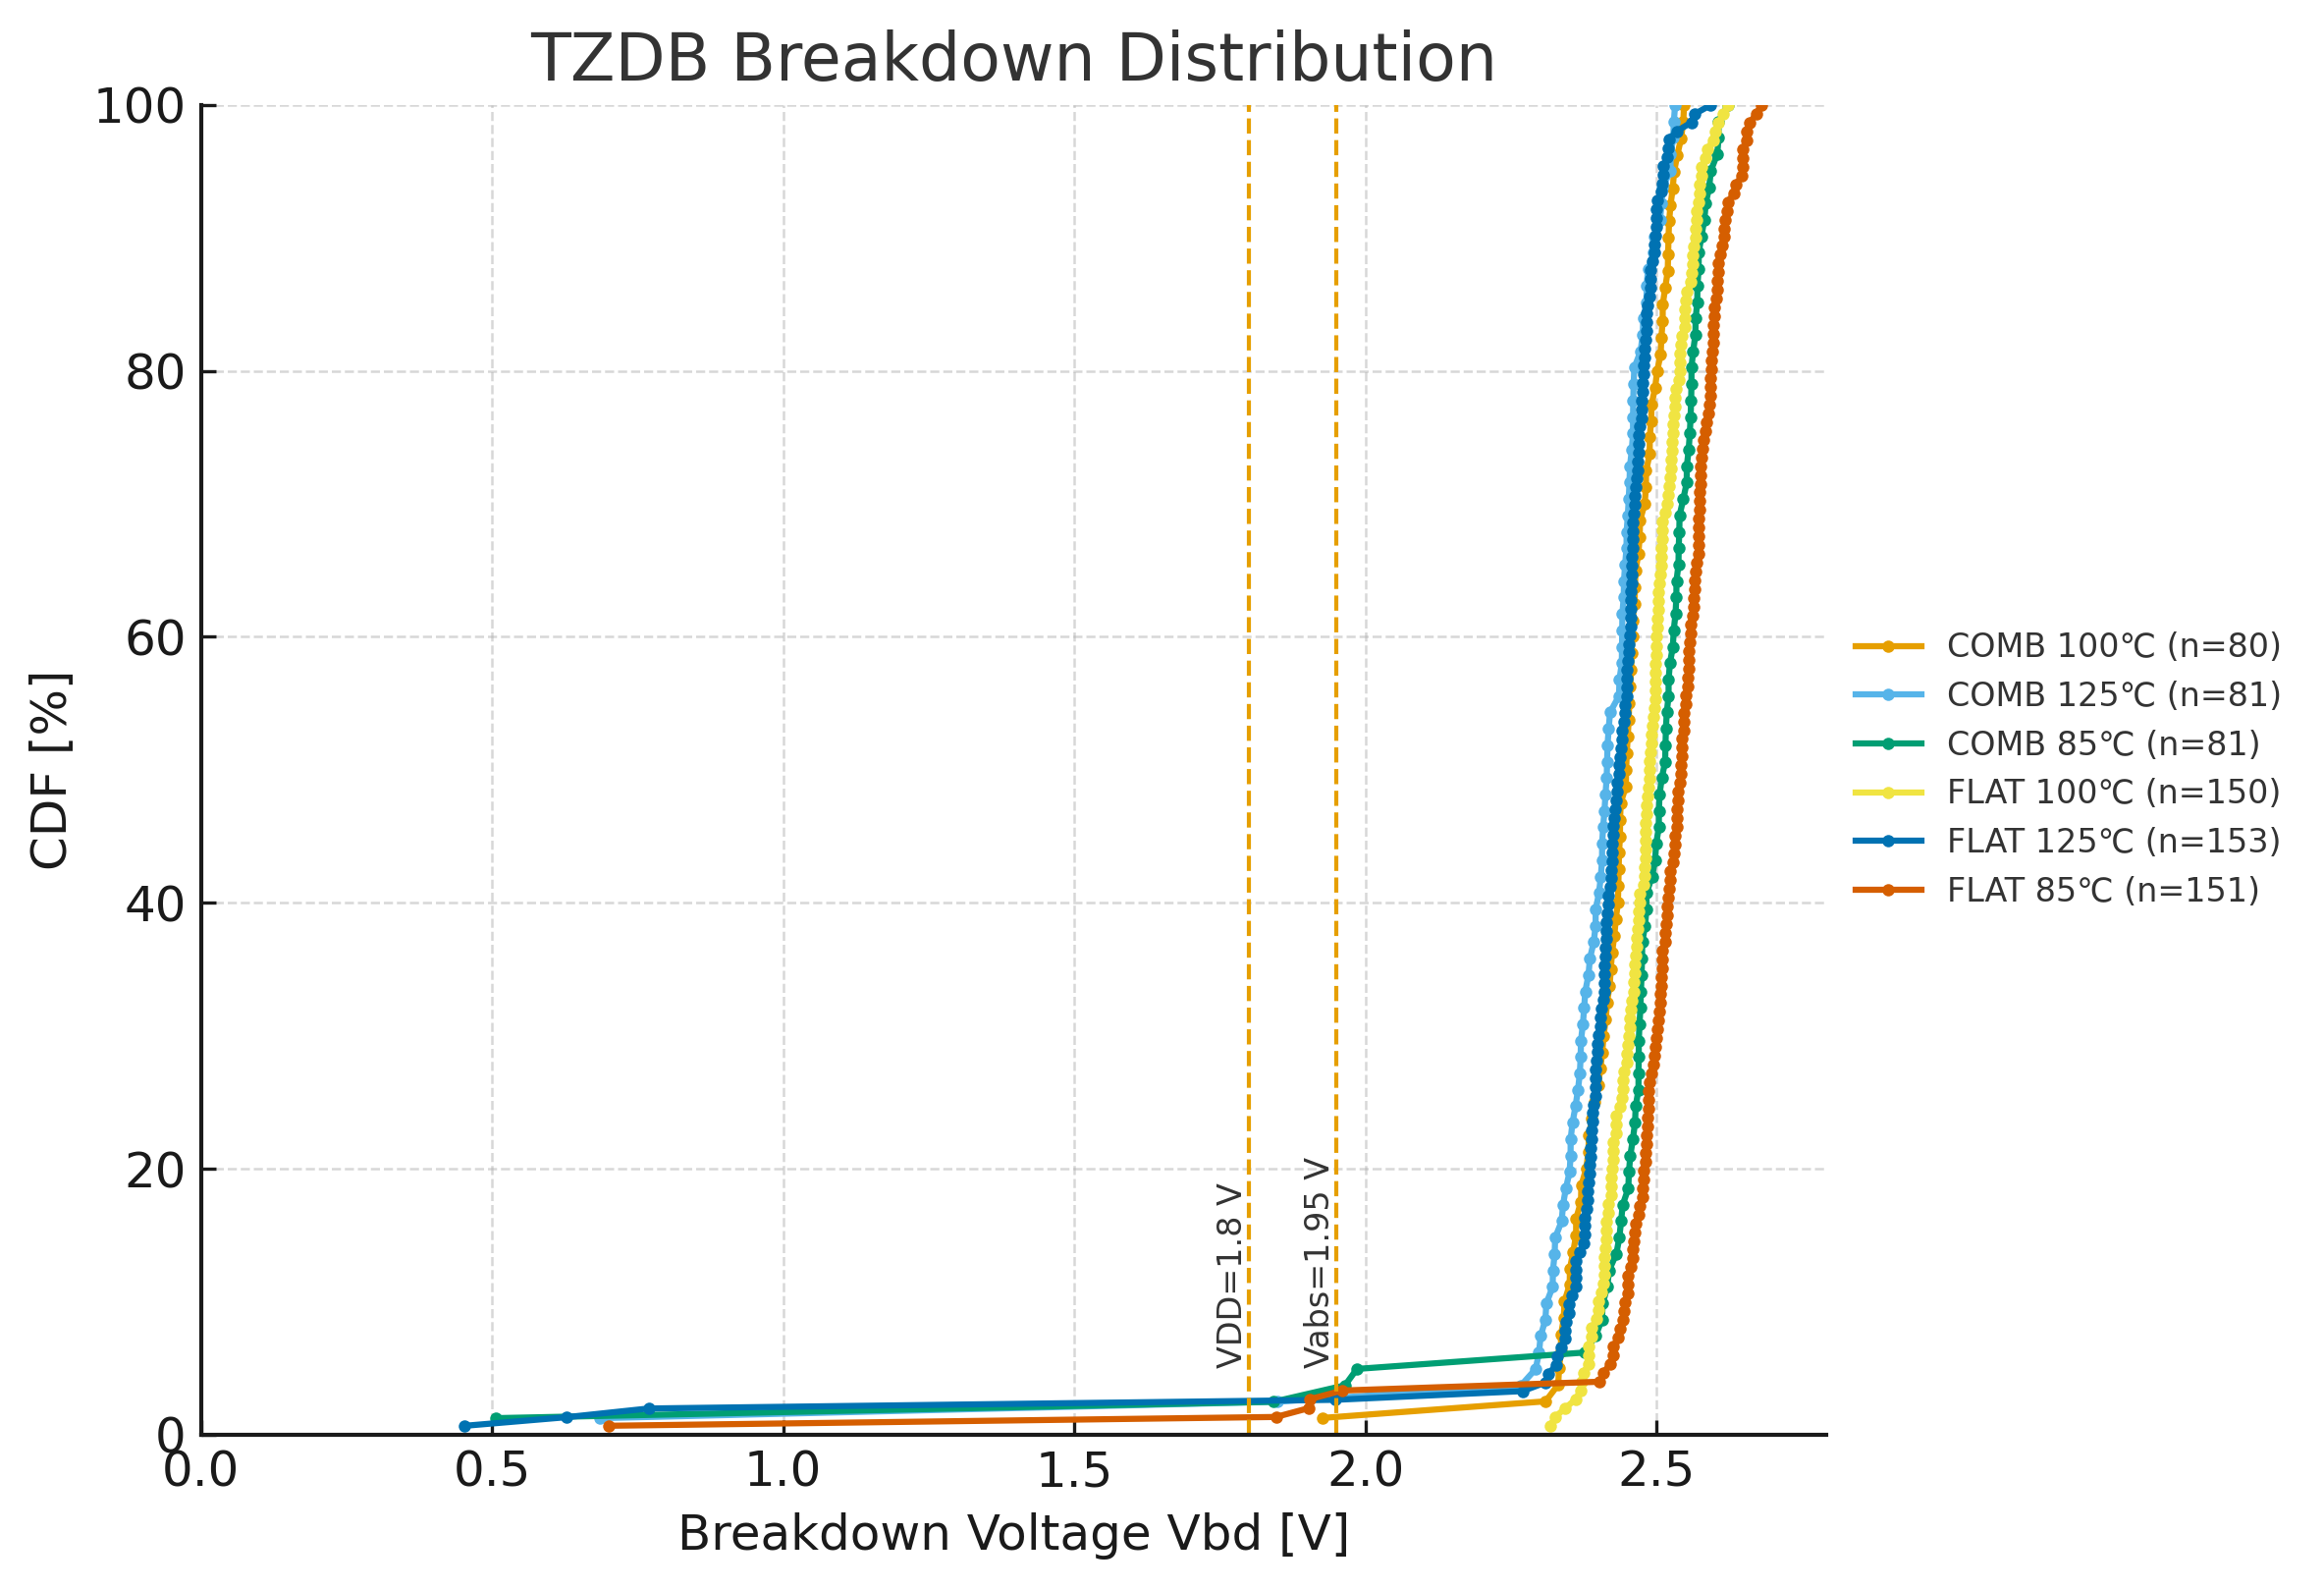
\includegraphics[width=0.48\linewidth]{figures/fig3_tzdb.png}}\hfill
  \subfloat[TDDB Weibull plots with fitted lines $(\beta,\eta)$.]{
    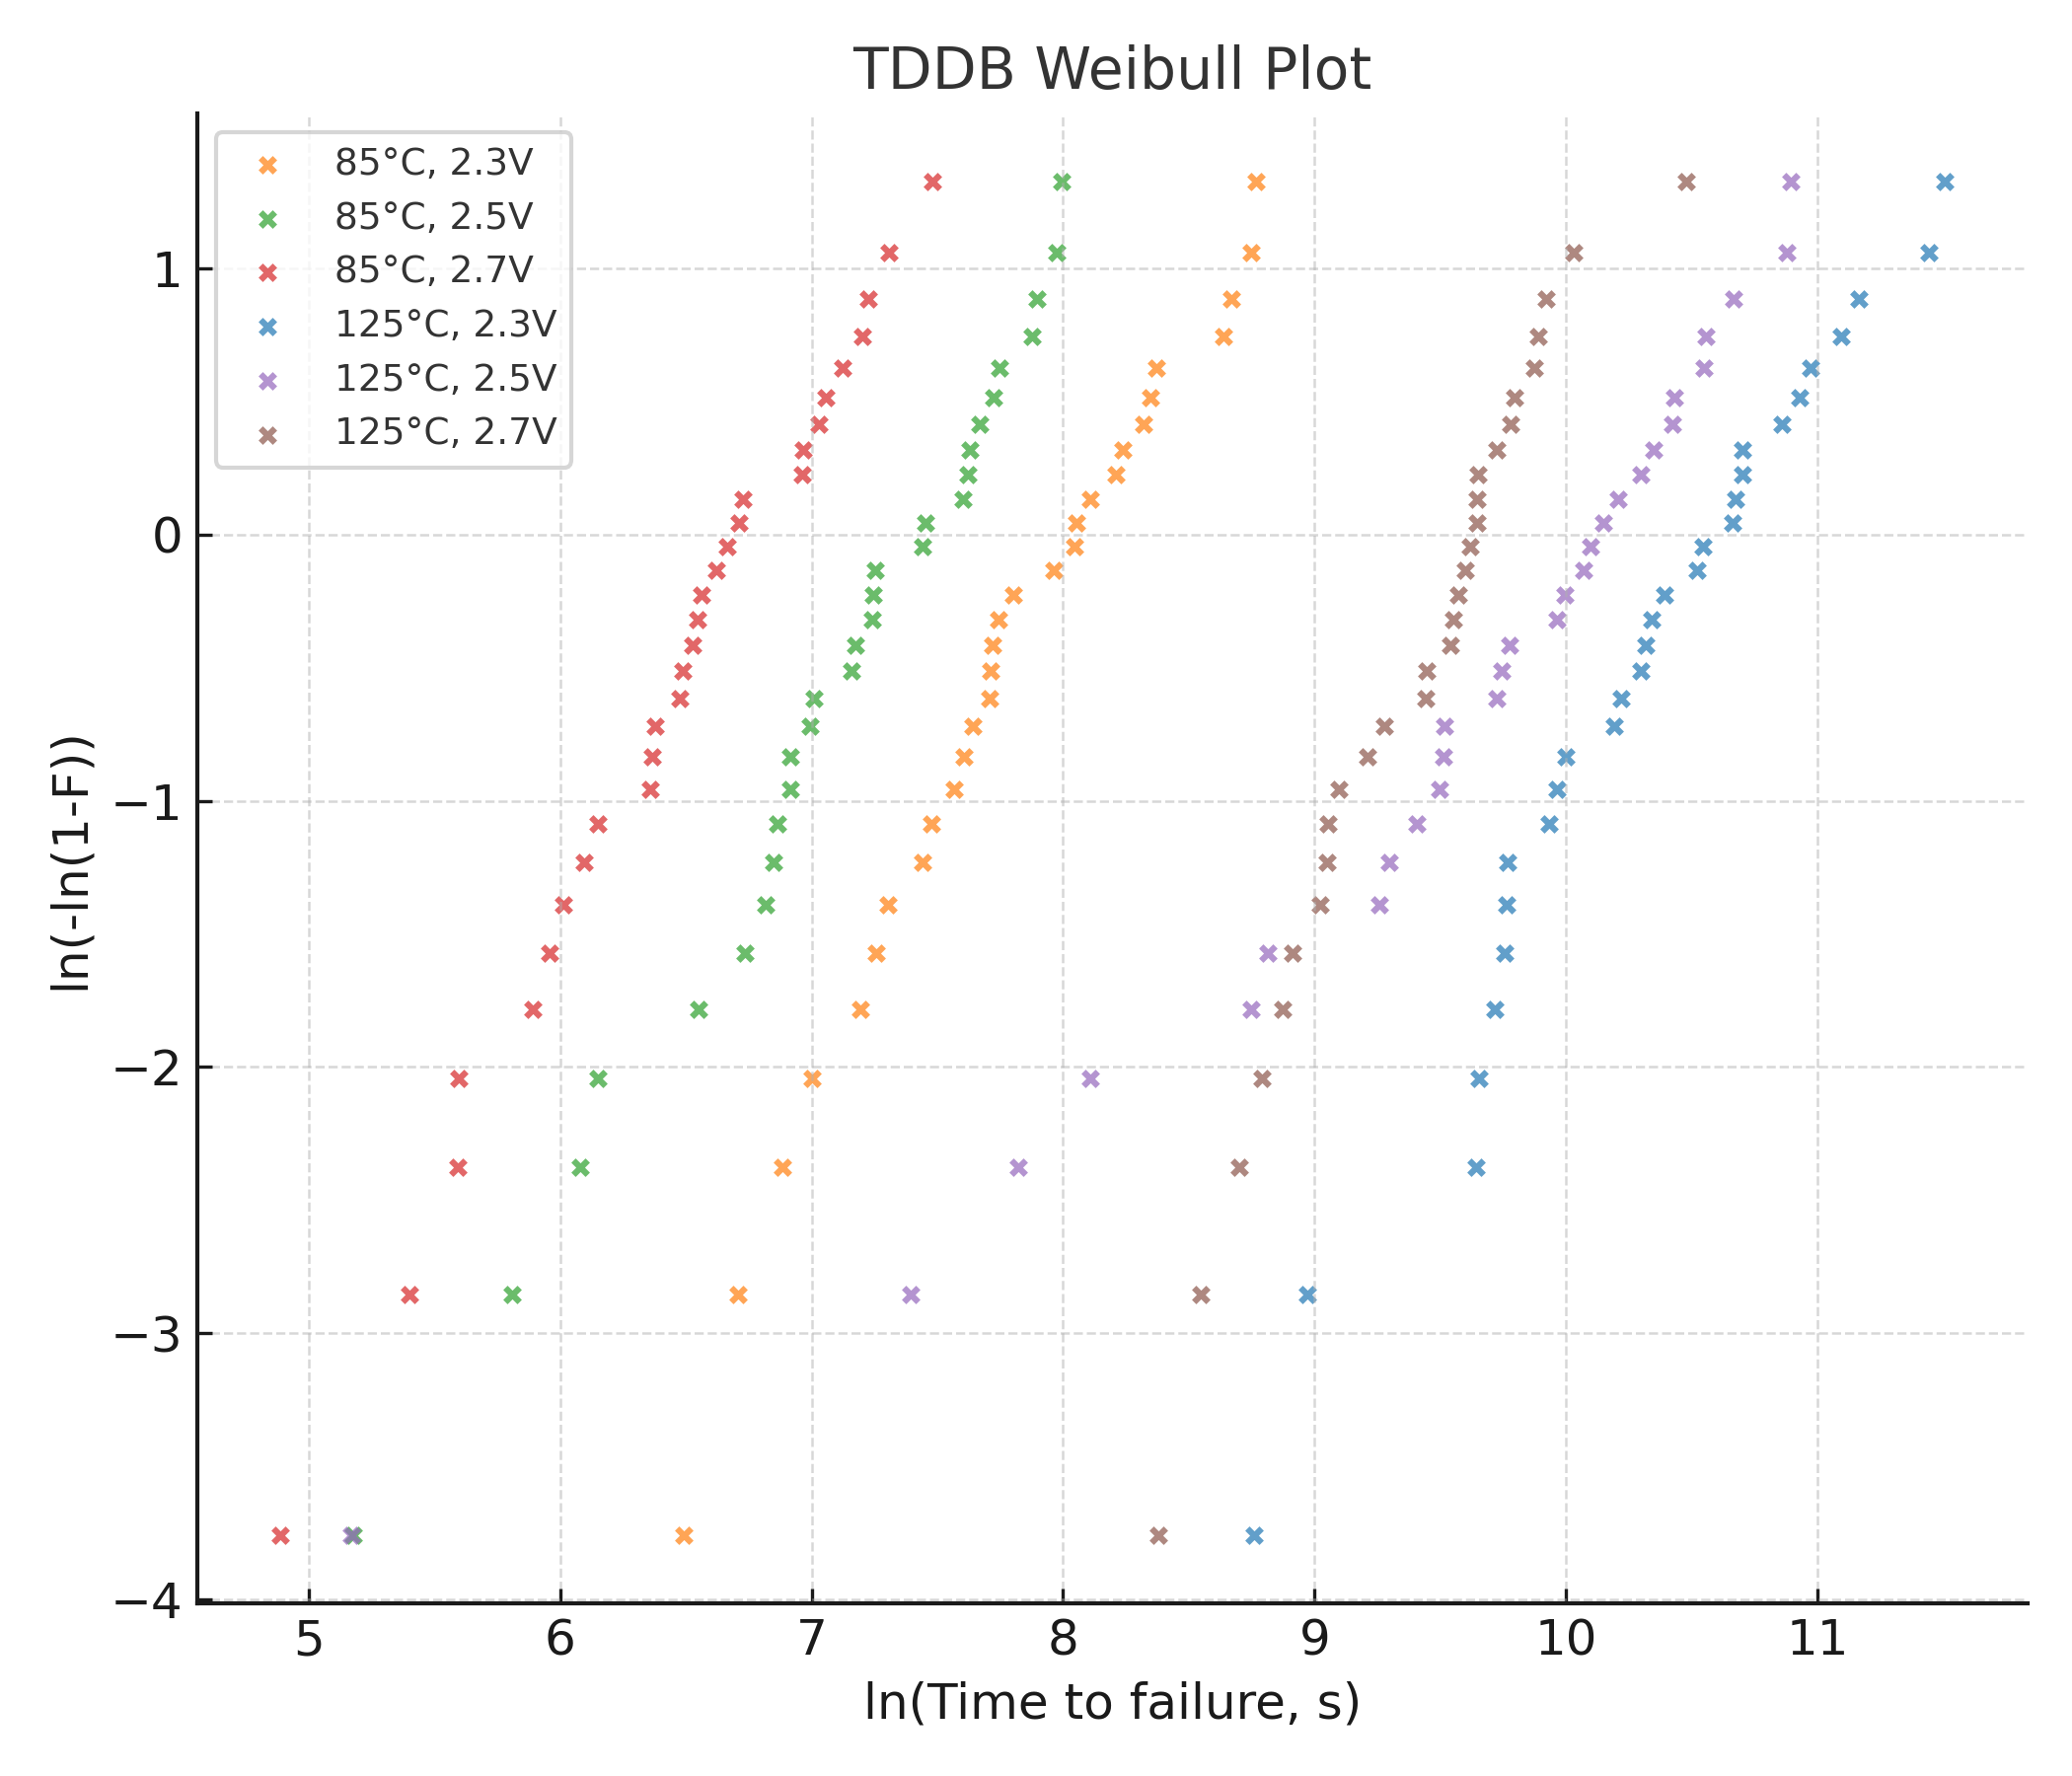
\includegraphics[width=0.48\linewidth]{figures/fig4_tddb_weibull.png}}\\[0.6ex]
  \subfloat[TDDB CDF under all stress conditions.]{
    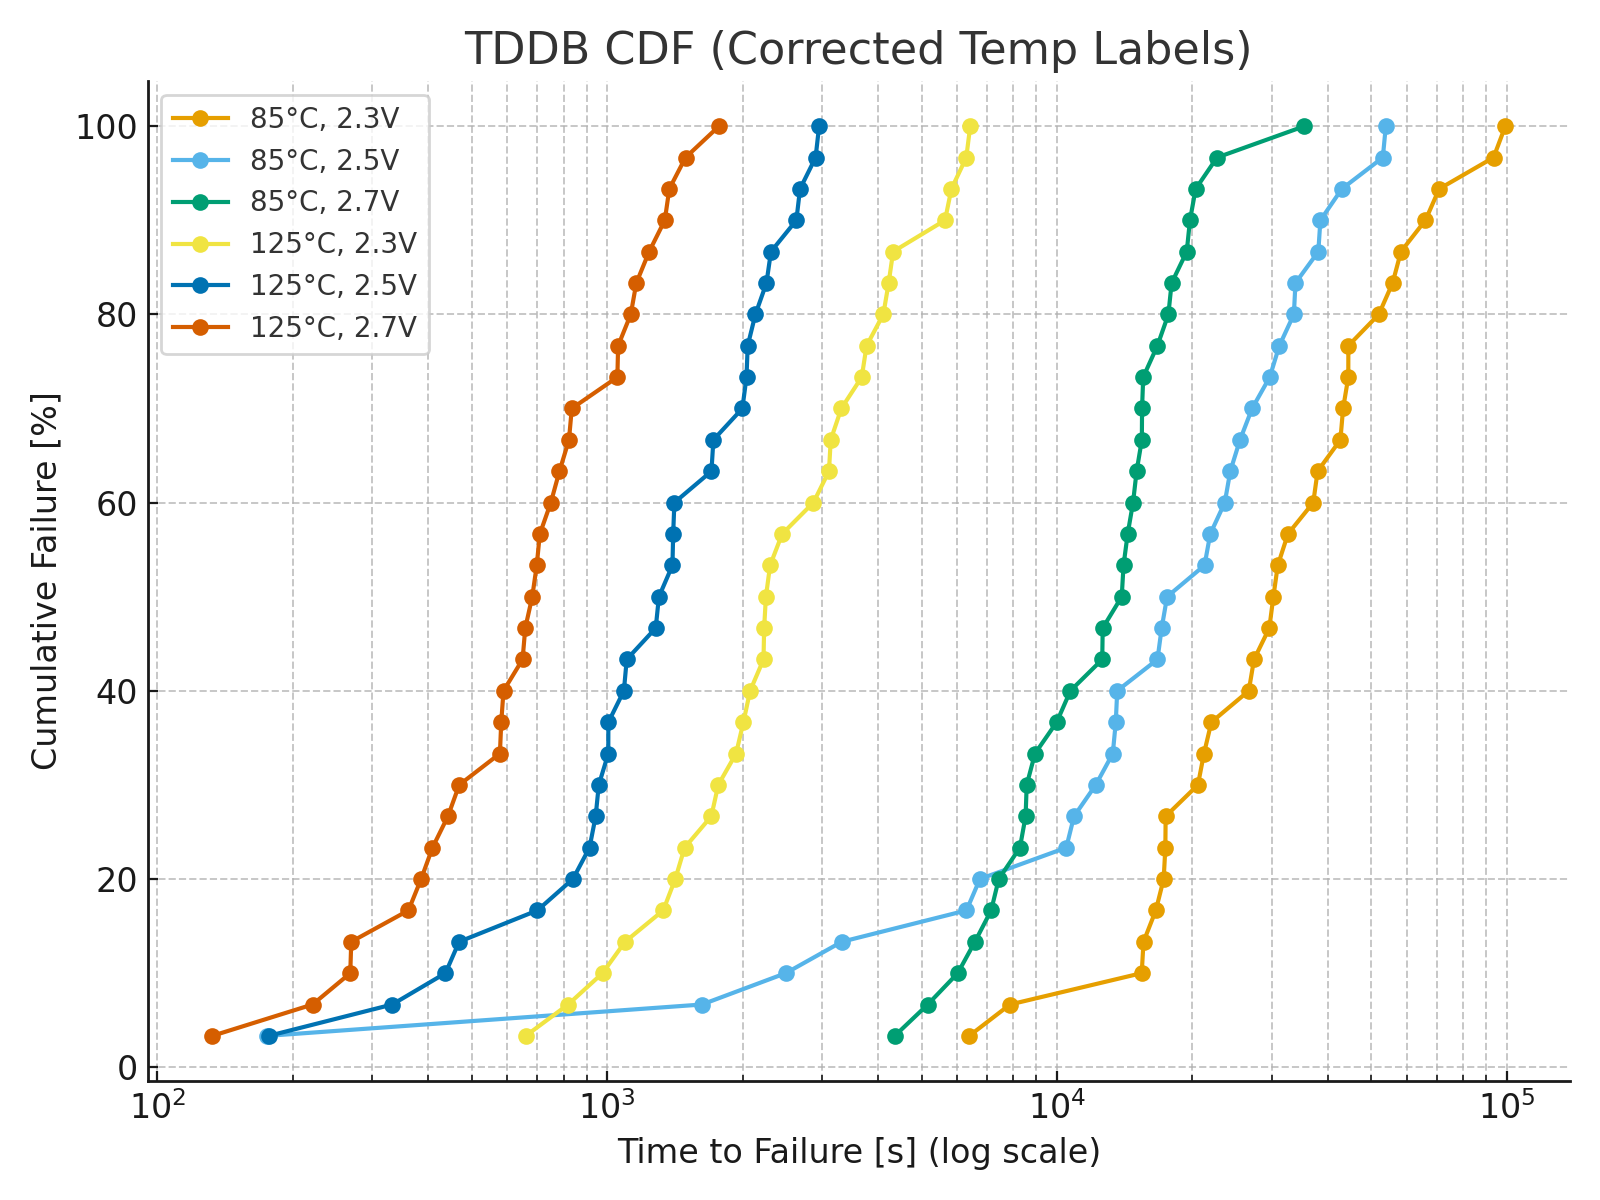
\includegraphics[width=0.48\linewidth]{figures/fig4_tddb_cdf.png}}\hfill
  \subfloat[Endurance characteristics $(\Delta V_{\mathrm{th}}$ vs. cycles).]{
    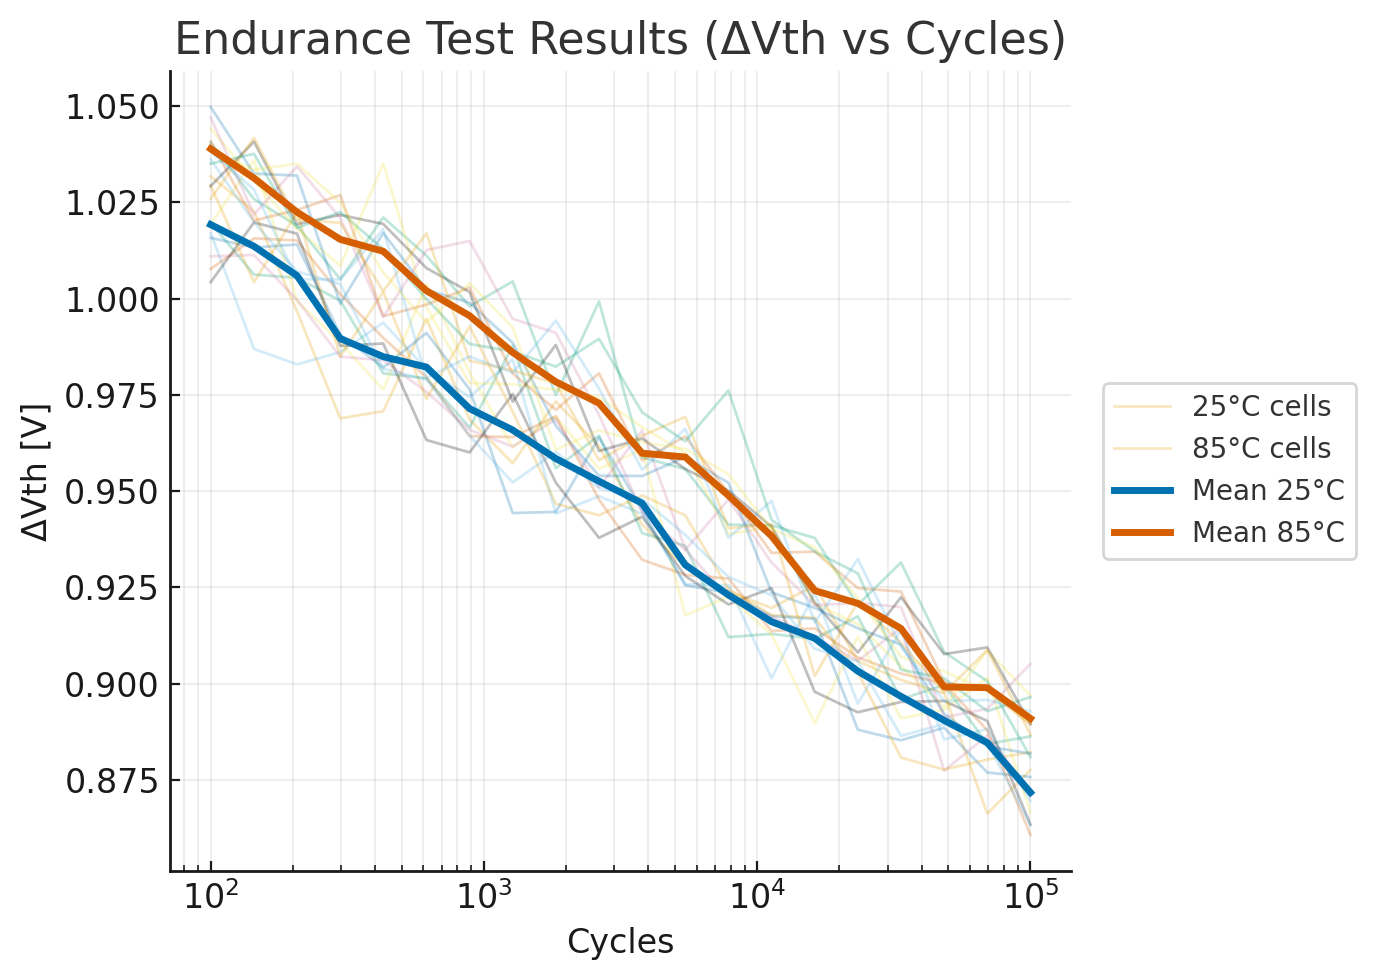
\includegraphics[width=0.48\linewidth]{figures/fig5_endurance.png}}
  \caption{Reliability results summary.}
  \label{fig:reliab_block}
\end{figure*}

\subsection{TDDB (Weibull/Arrhenius)}
Weibull plots yield $\beta \approx 1.3$. 
Arrhenius analysis gives activation energies consistent with oxygen-vacancy diffusion: 
$E_a \approx 0.78$ eV @ 2.3 V, 0.84 eV @ 2.5 V, 0.88 eV @ 2.7 V.

\subsection{Endurance}
Up to $10^5$ cycles verified; the window shrinks 20–30\%. 
A compact fit is $\Delta V_{\mathrm{th}}(N) = 1.12 - 0.05 \log_{10} N$.

\subsection{Retention}
Arrhenius extrapolation with $E_a \approx 1.1$ eV predicts: $>$100 years @ 25$^\circ$C, $>$10 years @ 85$^\circ$C, and only months @ 150$^\circ$C.

\tightsecspace
\section{System Architecture (SRAM + FeFET)}
The SoC uses a single 1.8 V core domain for logic, SRAM, and FeFET access.
Write/erase pulses ($\pm$2.3–2.7 V, 1–50 $\mu$s) are generated by an on-chip charge pump.
A lightweight backup controller copies SRAM contents to the FeFET array on power-fail detection and restores them at power-up.
An optional 3.3 V peripheral domain is kept for I/O and AMS (ADC/DAC, LDO).

\begin{figure}[!t]
  \centering
  \resizebox{0.95\columnwidth}{!}{%
    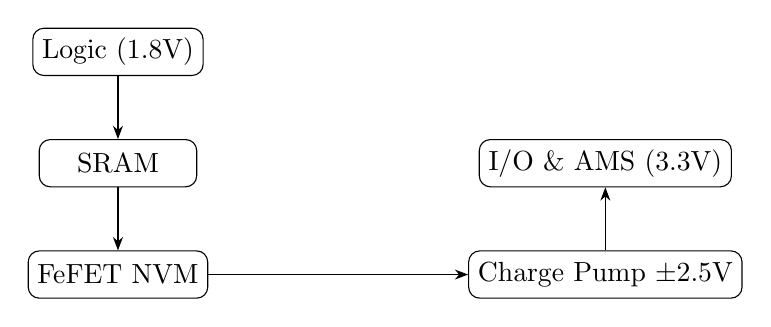
\begin{tikzpicture}[node distance=8mm, every node/.style={draw,rounded corners,minimum width=20mm,minimum height=6mm,align=center},>=Stealth,transform shape]
      \node (logic) {Logic (1.8V)};
      \node (sram) [below=of logic] {SRAM};
      \node (fefet) [below=of sram] {FeFET NVM};
      \node (pump) [right=of fefet, xshift=25mm] {Charge Pump $\pm$2.5V};
      \node (io) [above=of pump] {I/O \& AMS (3.3V)};
      \draw[->] (logic) -- (sram);
      \draw[->] (sram) -- (fefet);
      \draw[->] (fefet) -- (pump);
      \draw[->] (pump) -- (io);
    \end{tikzpicture}}
  \caption{System architecture with SRAM + FeFET backup.}
  \label{fig:system}
\end{figure}

% ==== Fig.5: Backup/restore flow ====
\begin{figure}[!t]
  \centering
  \resizebox{0.95\columnwidth}{!}{%
  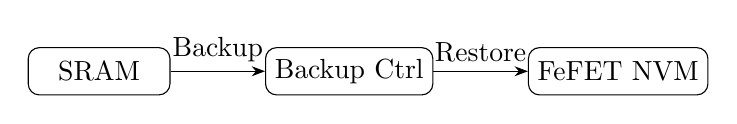
\begin{tikzpicture}[
      node distance=8mm,
      box/.style={draw,rounded corners,minimum width=18mm,minimum height=6mm}
  ]
    \node[box] (sram) {SRAM};
    \node[box, right=12mm of sram] (ctrl) {Backup Ctrl};
    \node[box, right=12mm of ctrl] (nvm)  {FeFET NVM};

    \draw[-{Stealth}] (sram) -- node[above,sloped]{Backup} (ctrl);
    \draw[-{Stealth}] (ctrl) -- node[above,sloped]{Restore} (nvm);
  \end{tikzpicture}}
  \caption{Backup/restore flow between SRAM and FeFET.}
  \label{fig:backup_flow}
\end{figure}

\section{Discussion}
The HZO/Al$_2$O$_3$/TiN stack provides sufficient reliability for industrial/consumer embedded NVM. 
For high-temperature automotive, improvements are required: IL optimization, crystallinity control, refresh/rewrite, and ECC.

\section{Conclusion}
We realized an FeFET module on 0.18~$\mu$m CMOS with one extra mask and one ALD tool. 
Devices exhibit $>10^5$ cycles and $>10$ years retention at 85$^\circ$C. 
The method extends mature-node lifetime and enables cost-effective embedded NVM for automotive/industrial/IoT.

\section*{Acknowledgment}
The author thanks collaborators for helpful discussions.

% --- 段落揃え用 ---
\IEEEtriggeratref{5}

\begin{thebibliography}{1}
\bibitem{boscke2011} T. Böscke et al., Appl. Phys. Lett., vol. 99, p. 102903, 2011.
\bibitem{mueller2012} J. Müller et al., Appl. Phys. Lett., vol. 99, p. 112901, 2012.
\bibitem{mikolajick2019} T. Mikolajick et al., J. Appl. Phys., vol. 125, p. 204103, 2019.
\bibitem{mueller2015} J. Müller et al., IEEE Trans. Electron Devices, vol. 62, no. 12, pp. 4158–4166, 2015.
\bibitem{park2020} J. Park et al., IEEE Electron Device Lett., vol. 41, no. 5, pp. 711–714, 2020.
\bibitem{nakamura2003} H. Nakamura et al., IEEE Trans. Device Mater. Rel., vol. 3, no. 4, pp. 132–136, 2003.
\bibitem{yamazaki2018} K. Yamazaki et al., Jpn. J. Appl. Phys., vol. 57, 04FB07, 2018.
\end{thebibliography}

\section*{Biography}
Shinichi Samizo has over 25 years of experience in semiconductor process integration and actuator development. After studying control theory and EM modeling in academia, he joined Seiko Epson in 1997 and worked on 0.35–0.18~$\mu$m CMOS logic/memory/HV integration, DRAM, and LCD drivers. Later he contributed to PZT actuator development and the PrecisionCore inkjet head. He is currently an independent researcher, publishing educational materials via the ``Project Design Hub''.

\end{document}
